% Token Service Cross-Period Pricing & Demand Response Game Framework
% Compile: xelatex framework_tikz.tex
\documentclass[tikz,border=5pt]{standalone}
\usepackage{xcolor,amsmath,amssymb}
\usetikzlibrary{shapes,arrows,positioning,fit,calc}

\definecolor{prussian}{HTML}{1B3A5C}
\definecolor{teal}{HTML}{007C7C}
\definecolor{orange}{HTML}{E07A2B}
\definecolor{green}{HTML}{2D8B4E}
\definecolor{lightbg}{HTML}{D6E4F0}
\definecolor{darkgray}{HTML}{333333}

\begin{document}
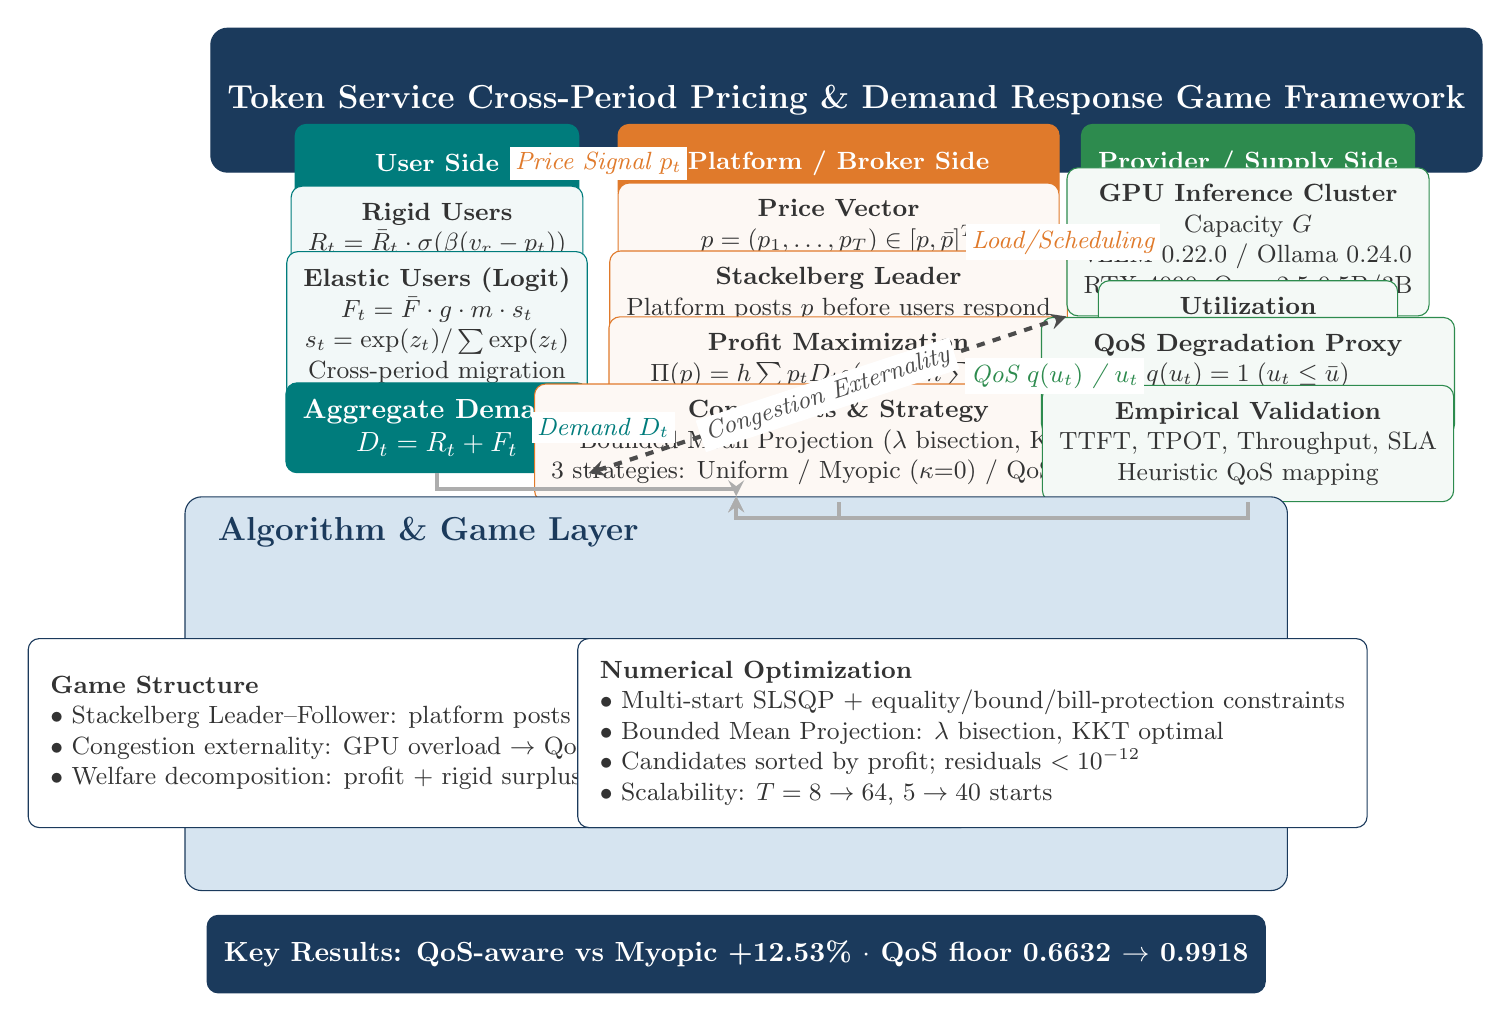
\begin{tikzpicture}[
    font=\sffamily,
    box/.style={rounded corners=4pt, draw, align=center, inner sep=6pt, text=darkgray, font=\small},
    header/.style={box, text=white, font=\bfseries\small},
    title/.style={box, text=white, font=\bfseries\large, fill=prussian, draw=prussian, minimum height=52pt, rounded corners=6pt},
    algo-box/.style={box, fill=white, draw=prussian, align=left, inner sep=8pt},
    arrow/.style={->, >=stealth, line width=1.5pt},
    darrow/.style={<->, >=stealth, line width=1.5pt, dashed},
    label/.style={font=\small\itshape, fill=white, inner sep=2pt}
]

% Column Positions
\pgfmathsetmacro{\cw}{3.6}
\pgfmathsetmacro{\cwm}{5.6}
\pgfmathsetmacro{\cwr}{3.8}
\pgfmathsetmacro{\cs}{0.5}
\pgfmathsetmacro{\lx}{0}
\pgfmathsetmacro{\mx}{\lx + \cw + \cs}
\pgfmathsetmacro{\rx}{\mx + \cwm + \cs}

% ── TITLE ──
\node[title, minimum width=14cm] (title) at (7cm, 0)
    {Token Service Cross-Period Pricing \& Demand Response Game Framework};

% ── COLUMN HEADERS ──
\node[header, fill=teal, draw=teal, minimum width=\cw cm, minimum height=28pt]
    (userH) at ($(\lx, -0.8) + (\cw/2, 0)$) {User Side};
\node[header, fill=orange, draw=orange, minimum width=\cwm cm, minimum height=28pt]
    (platformH) at ($(\mx, -0.8) + (\cwm/2, 0)$) {Platform / Broker Side};
\node[header, fill=green, draw=green, minimum width=\cwr cm, minimum height=28pt]
    (providerH) at ($(\rx, -0.8) + (\cwr/2, 0)$) {Provider / Supply Side};

% ── USER SIDE ──
\node[box, fill=teal!5, draw=teal, minimum width=\cw cm]
    (rigid) at ($(userH.south) + (0, -0.5)$)
    {\textbf{Rigid Users}\\
     $R_t = \bar{R}_t \cdot \sigma(\beta(v_r - p_t))$\\
     Price-sensitive demand};

\node[box, fill=teal!5, draw=teal, minimum width=\cw cm]
    (elastic) at ($(rigid.south) + (0, -0.35)$)
    {\textbf{Elastic Users (Logit)}\\
     $F_t = \bar{F} \cdot g \cdot m \cdot s_t$\\
     $s_t = \exp(z_t) / \sum \exp(z_t)$\\
     Cross-period migration};

\node[box, fill=teal, text=white, draw=teal, minimum width=\cw cm, font=\bfseries]
    (agg) at ($(elastic.south) + (0, -0.35)$)
    {\textbf{Aggregate Demand}\\
     $D_t = R_t + F_t$};

% ── PLATFORM SIDE ──
\node[box, fill=orange!5, draw=orange, minimum width=\cwm cm]
    (price) at ($(platformH.south) + (0, -0.5)$)
    {\textbf{Price Vector}\\
     $p = (p_1, \dots, p_T) \in [\underline{p}, \bar{p}]^T$\\
     Fixed mean: $\sum p_t / T = \bar{p}$};

\node[box, fill=orange!5, draw=orange, minimum width=\cwm cm]
    (stackel) at ($(price.south) + (0, -0.1)$)
    {\textbf{Stackelberg Leader}\\
     Platform posts $p$ before users respond\\
     Game-theoretic first-mover advantage};

\node[box, fill=orange!5, draw=orange, minimum width=\cwm cm]
    (profit) at ($(stackel.south) + (0, -0.1)$)
    {\textbf{Profit Maximization}\\
     $\Pi(p) = h\sum p_t D_t q(u_t) - h\sum w D_t$\\
     $- h\sum c_r(\bar{R}_t{-}R_t) - h\sum c_q[1{-}q(u_t)]R_t$};

\node[box, fill=orange!5, draw=orange, minimum width=\cwm cm]
    (strategy) at ($(profit.south) + (0, -0.1)$)
    {\textbf{Constraints \& Strategy}\\
     Bounded Mean Projection ($\lambda$ bisection, KKT)\\
     3 strategies: Uniform / Myopic ($\kappa{=}0$) / QoS-aware};

% ── PROVIDER SIDE ──
\node[box, fill=green!5, draw=green, minimum width=\cwr cm]
    (gpu) at ($(providerH.south) + (0, -0.5)$)
    {\textbf{GPU Inference Cluster}\\
     Capacity $G$\\
     vLLM 0.22.0 / Ollama 0.24.0\\
     RTX 4090, Qwen2.5-0.5B/3B};

\node[box, fill=green!5, draw=green, minimum width=\cwr cm]
    (util) at ($(gpu.south) + (0, -0.1)$)
    {\textbf{Utilization}\\
     $u_t = D_t / G$};

\node[box, fill=green!5, draw=green, minimum width=\cwr cm]
    (qos) at ($(util.south) + (0, -0.1)$)
    {\textbf{QoS Degradation Proxy}\\
     $q(u_t) = 1 \;(u_t \le \bar{u})$\\
     $q(u_t) = \exp[-\kappa(u_t-\bar{u})^2] \;(u_t > \bar{u})$};

\node[box, fill=green!5, draw=green, minimum width=\cwr cm]
    (emp) at ($(qos.south) + (0, -0.1)$)
    {\textbf{Empirical Validation}\\
     TTFT, TPOT, Throughput, SLA\\
     Heuristic QoS mapping};

% ── ARROWS ──
\draw[darrow, orange] ($(platformH.west)$) -- node[label, text=orange]{Price Signal $p_t$} ($(userH.east)$);
\draw[arrow, teal] ($(agg.east)$) -- node[label, text=teal]{Demand $D_t$} ($(agg.east -| price.west)$);
\draw[arrow, orange] ($(price.east)$) -- node[label, text=orange]{Load/Scheduling} ($(price.east -| gpu.west)$);
\draw[darrow, green] ($(qos.west)$) -- node[label, text=green]{QoS $q(u_t)$ / $u_t$} ($(qos.west -| profit.east)$);
\draw[darrow, gray!60!black] ($(agg.south east)$) -- node[label, text=gray!60!black, sloped]{Congestion Externality} ($(gpu.south west)$);

% ── ALGORITHM LAYER ──
\node[fill=lightbg, draw=prussian, rounded corners=6pt, minimum width=14cm, minimum height=5cm, inner sep=10pt]
    (algoBg) at ($(agg.south) + (3.8cm, -2.8cm)$) {};

\node[text=prussian, font=\bfseries\large, anchor=north west]
    at ($(algoBg.north west) + (0.3cm, -0.15cm)$) {Algorithm \& Game Layer};

\node[algo-box, minimum width=6cm, minimum height=2.4cm]
    (game) at ($(algoBg.center) + (-3cm, -0.5cm)$)
    {\textbf{Game Structure}\\
     $\bullet$ Stackelberg Leader--Follower: platform posts $p$, users respond via logit\\
     $\bullet$ Congestion externality: GPU overload $\to$ QoS $\downarrow$ $\to$ effective service $\downarrow$\\
     $\bullet$ Welfare decomposition: profit + rigid surplus + elastic log-sum $-$ carbon cost};

\node[algo-box, minimum width=6cm, minimum height=2.4cm]
    (opt) at ($(algoBg.center) + (3cm, -0.5cm)$)
    {\textbf{Numerical Optimization}\\
     $\bullet$ Multi-start SLSQP + equality/bound/bill-protection constraints\\
     $\bullet$ Bounded Mean Projection: $\lambda$ bisection, KKT optimal\\
     $\bullet$ Candidates sorted by profit; residuals $< 10^{-12}$\\
     $\bullet$ Scalability: $T=8\rightarrow 64$, $5\rightarrow 40$ starts};

% ── KEY RESULTS ──
\node[box, fill=prussian, text=white, draw=prussian, minimum width=10cm, minimum height=28pt, font=\bfseries]
    (results) at ($(algoBg.south) + (0, -0.8cm)$)
    {Key Results: QoS-aware vs Myopic \textbf{+12.53\%} $\cdot$ QoS floor 0.6632 $\to$ \textbf{0.9918}};

% ── CONNECTORS: Columns → Algorithm ──
\draw[arrow, darkgray!40] ($(agg.south)$) -- ($(agg.south)+(0,-0.2)$) -| ($(algoBg.north)$);
\draw[arrow, darkgray!40] ($(strategy.south)$) -- ($(strategy.south)+(0,-0.2)$) -| ($(algoBg.north)$);
\draw[arrow, darkgray!40] ($(emp.south)$) -- ($(emp.south)+(0,-0.2)$) -| ($(algoBg.north)$);

\end{tikzpicture}
\end{document}
